\documentclass[a4,12pt]{horizon-theme}
\usepackage{lipsum}
\usepackage{fontawesome5}
\usepackage{graphicx,url}
\usepackage{float}
\usepackage{amsmath}
\usepackage{booktabs}
\usepackage{makecell}
\usepackage{array}
\usepackage{multirow}
\usepackage{caption}
\usepackage{subcaption}
\usepackage{siunitx}
\usepackage{enumerate}
\usepackage{gensymb}
\usepackage{csvsimple}
\usepackage{tabularray}
\usepackage{stackengine}
\usepackage{xcolor, colortbl}
\usepackage[round]{natbib}
\usepackage{karnaugh-map}
\usepackage{stackengine}
% \usepackage{longtable}
\usepackage{minted}
\usepackage{fontawesome}

\strutlongstacks{T}

\BeforeBeginEnvironment{minted}{\vspace{-20pt}}


% Cover Config
% \configCover{<num. do exp.>}{<data>}{<título>}
\configCover{9}{30/06/2022}{Projeto de Semáforos de Trânsito}


\begin{filecontents*}{vcc1.csv}
pos,comp,vcc,gnd
C1,74190,16,8
C2,74153,16,8
\end{filecontents*}


\newenvironment{code}{\captionsetup{type=listing}}{}


\begin{document}
\horizonCover

\horizonTitle


\section{Introdução}
Uma FPGA é um circuito integrado criado para ser configurado por um projetista após sua fabricação com uma linguagem de descrição de hardware. Neste projeto, será usada uma FPGA na implementação da unidade de controle de um circuito digital controlador de semáforos. Já o fluxo de dados será implementado utilizando circuitos integrados não programáveis.


\section{Objetivos}
O objetivo deste projeto é construir um circuito digital para controle de um sistema de semáforos em um cruzamento de duas vias de trânsito com as seguintes características:
\begin{itemize}
    \item controle de 2 semáforos ($S_0$ e $S_1$) com 6 transições de luzes no total
    \item tempo da duração de cada transição de sinal ajustável durante o funcionamento do semáforo (valor mínimo: 2, valor máximo: 4, ou seja 3 possibilidades)
    \item mesma duração para sinais iguais em semáforos diferentes
\end{itemize}

% \newpage
\section{Planejamento}
\subsection{Descrição Funcional}

Este circuito digital foi projetado para controlar os estados de dois semáforos em um cruzamento. A Fig. \ref{fig:semaforos} mostra a transição de todos os estados dos semáforos $S_0$ e $S_1$ com os respectivos tempos de transição entre cada estado, $T_0$, $T_1$ e $T_2$ que podem ser programados pelo usuário final. Em que $T_0$ é a duração do sinal verde/vermelho, $T_1$ é a duração do sinal amarelo/vermelho e $T_2$ é a duração do sinal vermelho/vermelho. Este tempo é um valor que pode ser configurado no momento da execução do circuito e é projetado para ter um valor entre 2 e 4, ou seja, o tempo de duração, na realidade, será o tempo programado acrescido de 1. Isto é, este circuito não foi projetado para ``pular'' estados.

\begin{figure}[!ht]
    \centering
    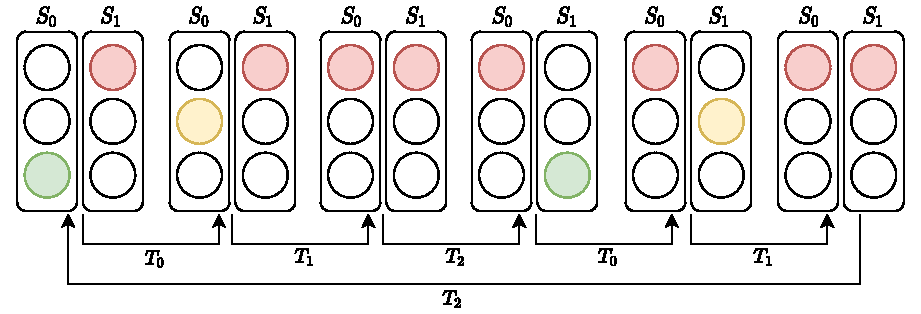
\includegraphics[width=\textwidth]{luzes.pdf}
    \caption{Transição de luzes dos semáforos $S_0$ e $S_1$ com seus respectivos tempos de transição}
    \label{fig:semaforos}
\end{figure}

\newpage
A Fig. \ref{fig:cruzamento} apresenta um esquema da disposição dos semáforos no cruzamento, indicando que o semáforo $S_0$ controla o fluxo Sul-Norte e o semáforo $S_1$ controla o fluxo Leste-Oeste.

\begin{figure}[!ht]
    \centering
    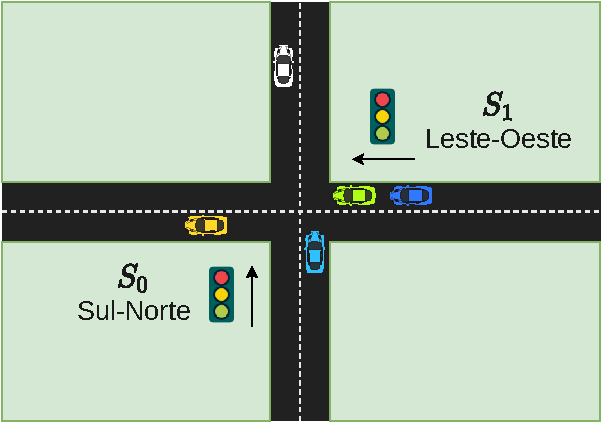
\includegraphics[width=0.75\textwidth]{cruzamento.pdf}
    \caption{Esboço da disposição dos semáforos no cruzamento indicando a orientação do fluxo de veículos controlado por cada semáforo}
    \label{fig:cruzamento}
\end{figure}



\subsection{Diagrama de Blocos}

A Fig. \ref{fig:blocos} mostra o diagrama de blocos do circuito controlador de semáforos. O cirucito recebe os sinais  de clock, reset e dos tempos de cada sinal e obtêm como saída um sinal de ativação para cada lâmpada dos dois semáforos. O Fluxo de Dados é composto por apenas um contador de 4 bits 74190, um multiplexador (74153) e a Unidade de Controle controla esse contador a partir do sinal load e os sinais de dados.

\begin{figure}[!ht]
    \centering
    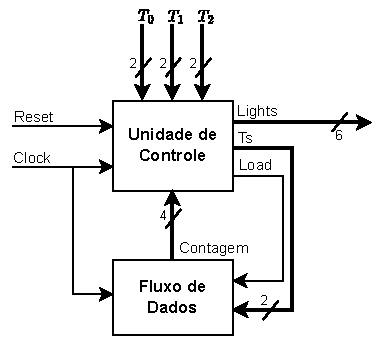
\includegraphics[width=.65\textwidth]{blocos.pdf}
    \caption{Diagrama de blocos do circuito controlador de semáforo}
    \label{fig:blocos}
\end{figure}


% \newpage
\subsection{Diagrama Lógico}

\begin{figure}[!ht]
    \centering
    \stackinset{r}{1pt}{b}{1pt}{\carimboA{Semáforo}}{%
        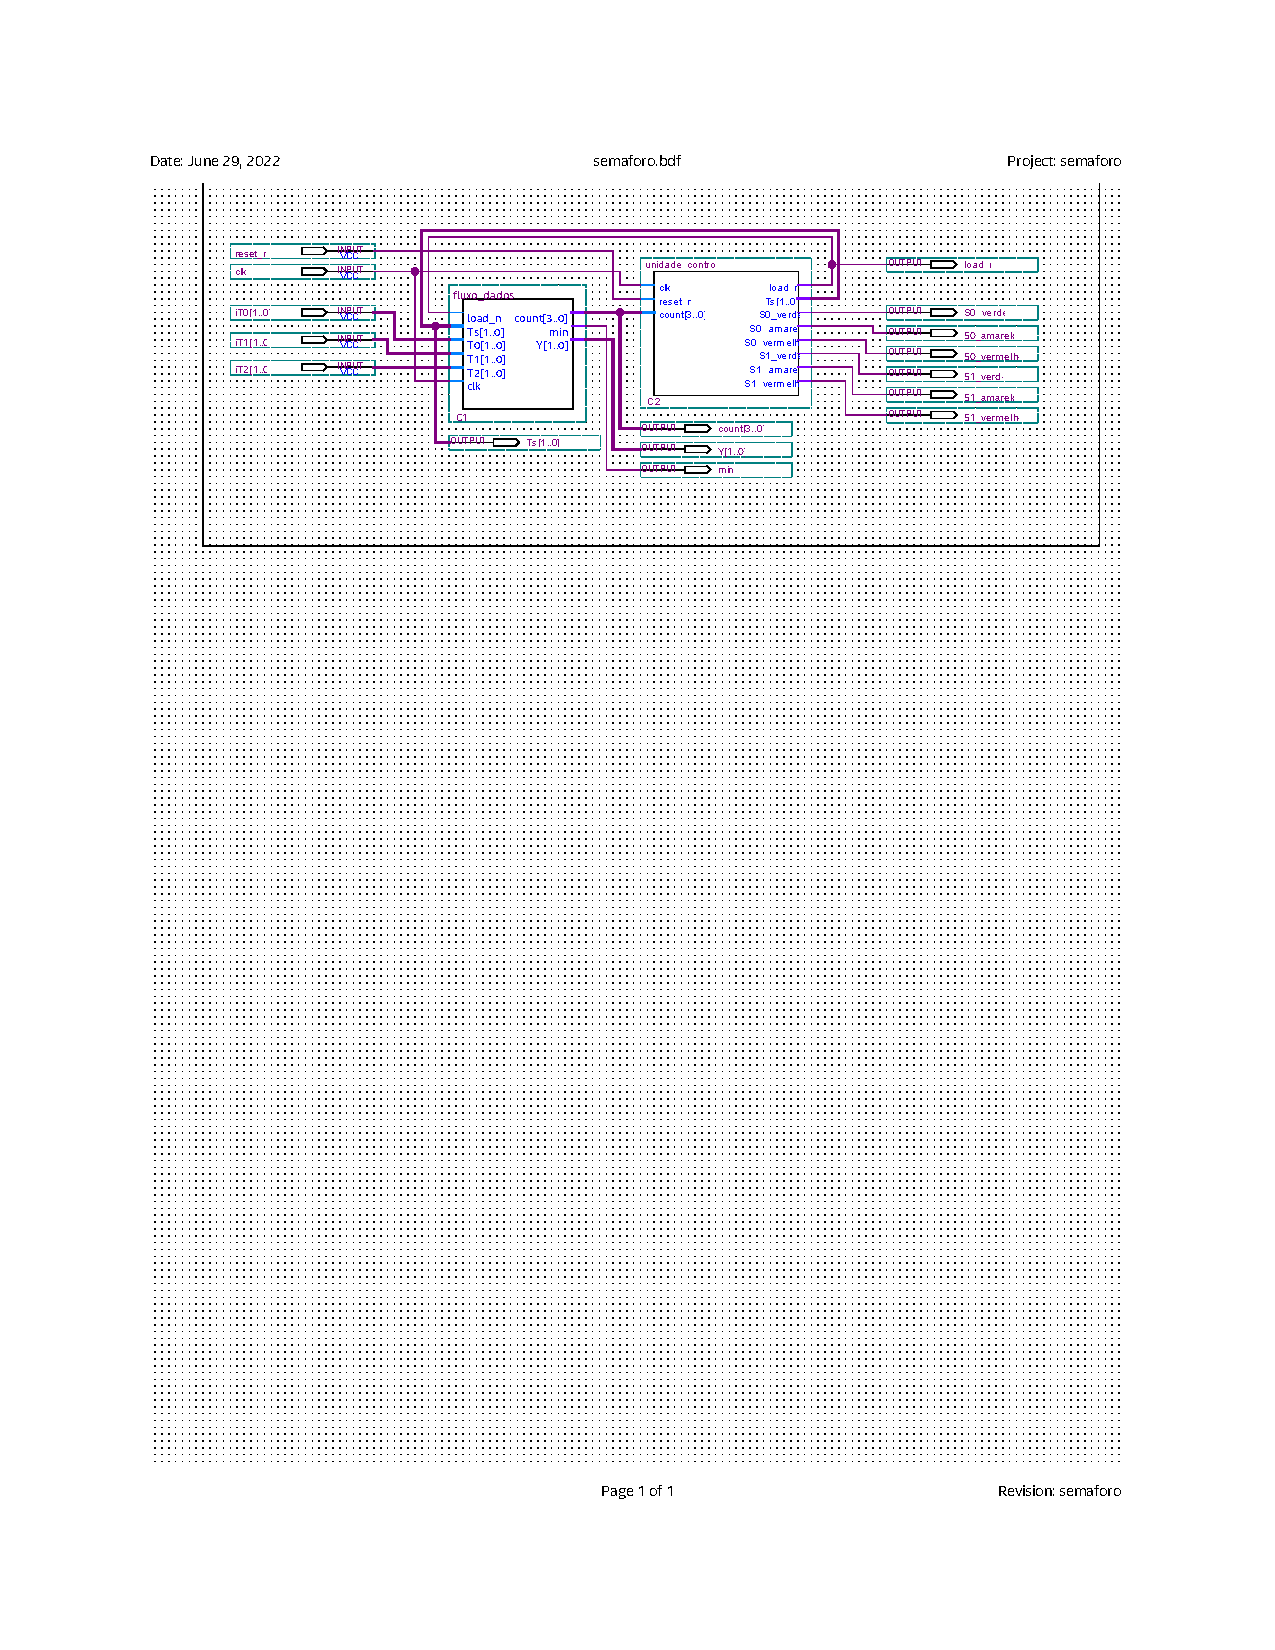
\includegraphics[width=\textwidth, trim={35mm, 188mm, 35mm, 35mm}, clip]{semaforo.pdf}%
    }
    \caption{Diagrama lógico do circuito completo, incluindo Fluxo de Dados e Unidade de Controle}
    \label{fig:logico}
\end{figure}

A Fig. \ref{fig:logico} mostra a implementação do circuito digital, que é constituído de dois blocos prinicipais: o fluxo de dados e a unidade de controle. O fluxo de dados é composto por um Contador de 4 bits 74190 e um multiplexador 74153, cujo diagrama lógico é mostrado na Fig. \ref{fig:logico_fd} e a unidade de controle é uma máquina de estados implementada em VHDL, cuja descrição é mostrada na Listagem \ref{lst:uc}.

\begin{figure}[!ht]
    \centering
    \stackinset{r}{1pt}{t}{1pt}{\carimboA{Semáforo (FD)}}{%
        \stackinset{r}{1pt}{b}{1pt}{\carimboB{vcc1.csv}}{%
            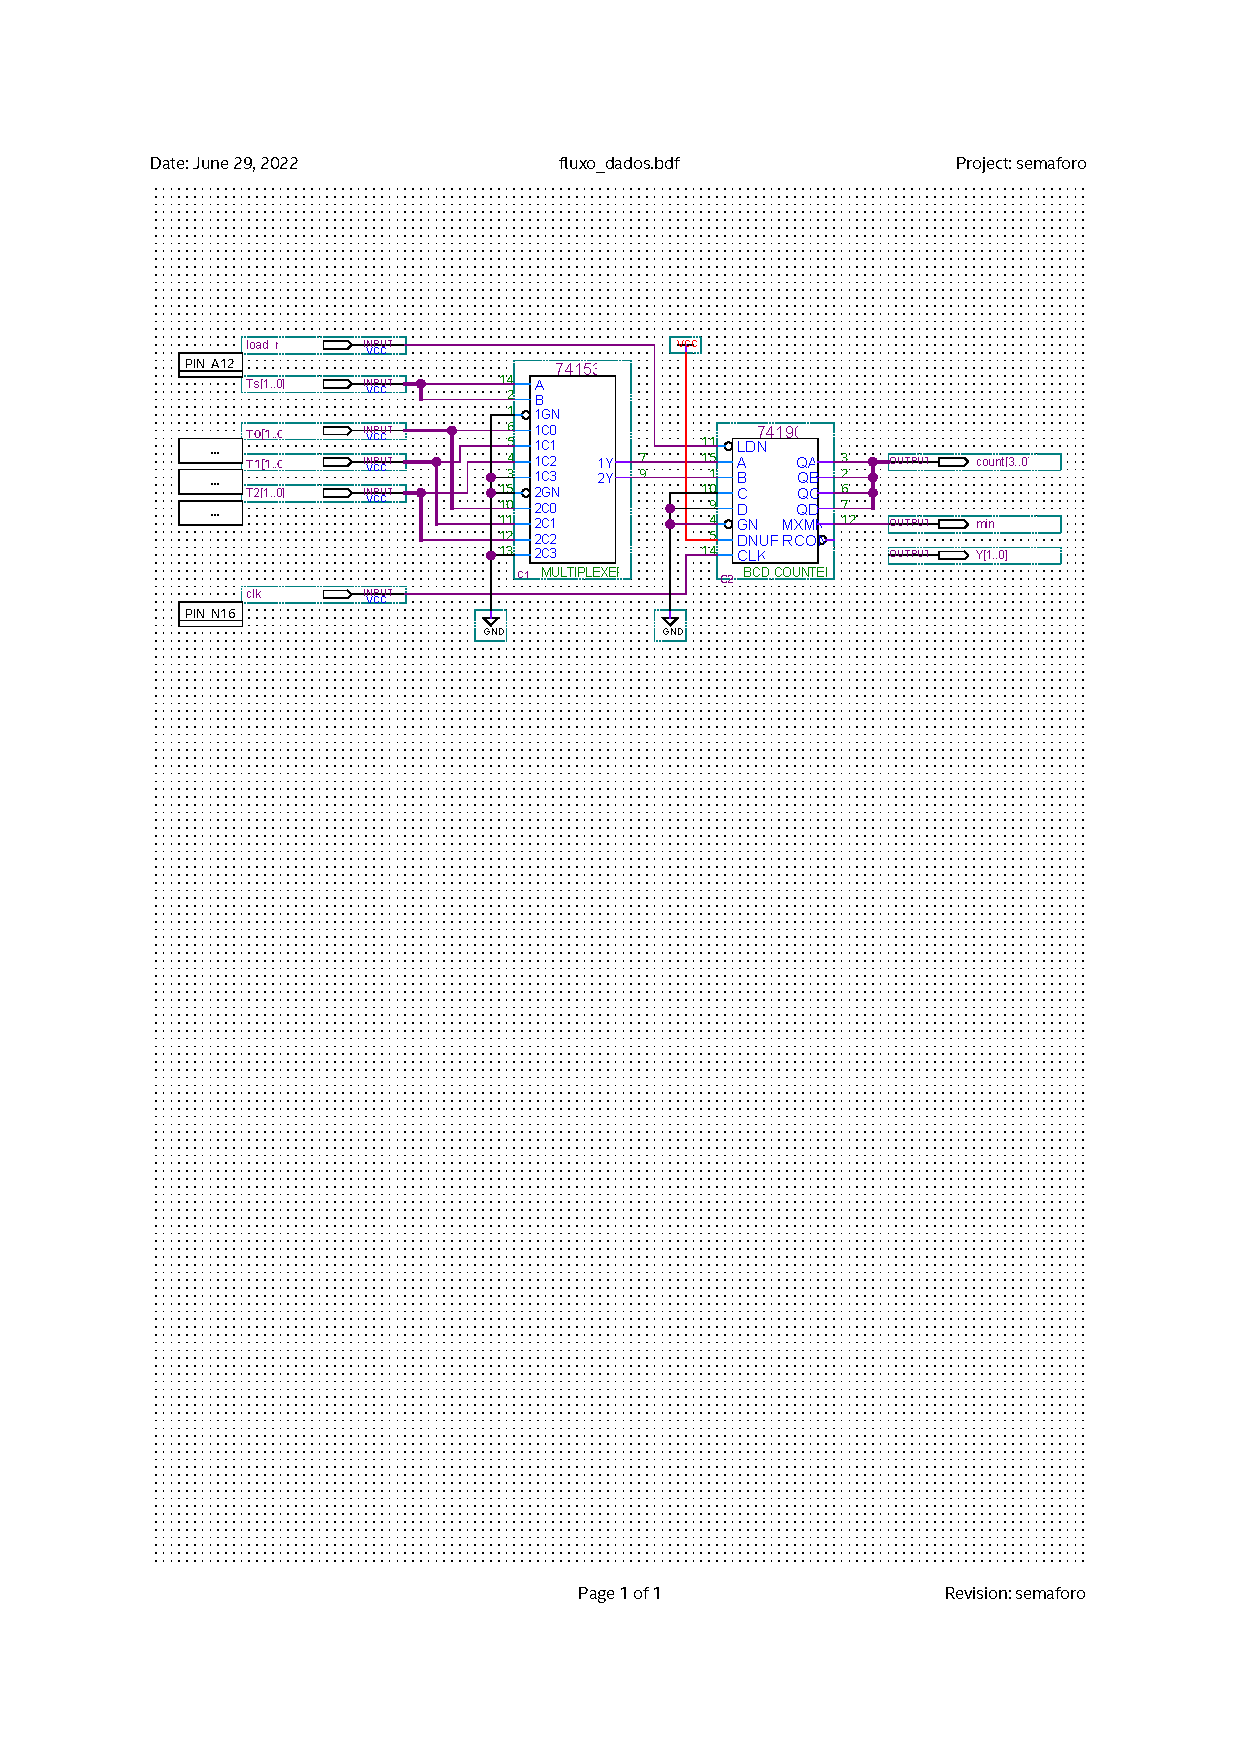
\includegraphics[width=\textwidth, trim={30mm, 188mm, 30mm, 55mm}, clip]{fluxo_dados.pdf}%
        }%
    }
    \caption{Diagrama lógico do Fluxo de Dados}
    \label{fig:logico_fd}
\end{figure}



\subsection{Diagrama de Estados}
A máquina de estados implementada na unidade de controle é composta por 12 estados. Os estados de carregamento $E0_L$ a $E5_L$ tem duranção de 1 clock e são acionados a cada troca de luzes do semáforo. Já os estados de contagem $E0_C$ a $E5_C$ representam a contagem dos 3 tempos de mudança de luzes dos semáforos mostrados na Fig. \ref{fig:semaforos}.

\begin{figure}[!ht]
    \centering
    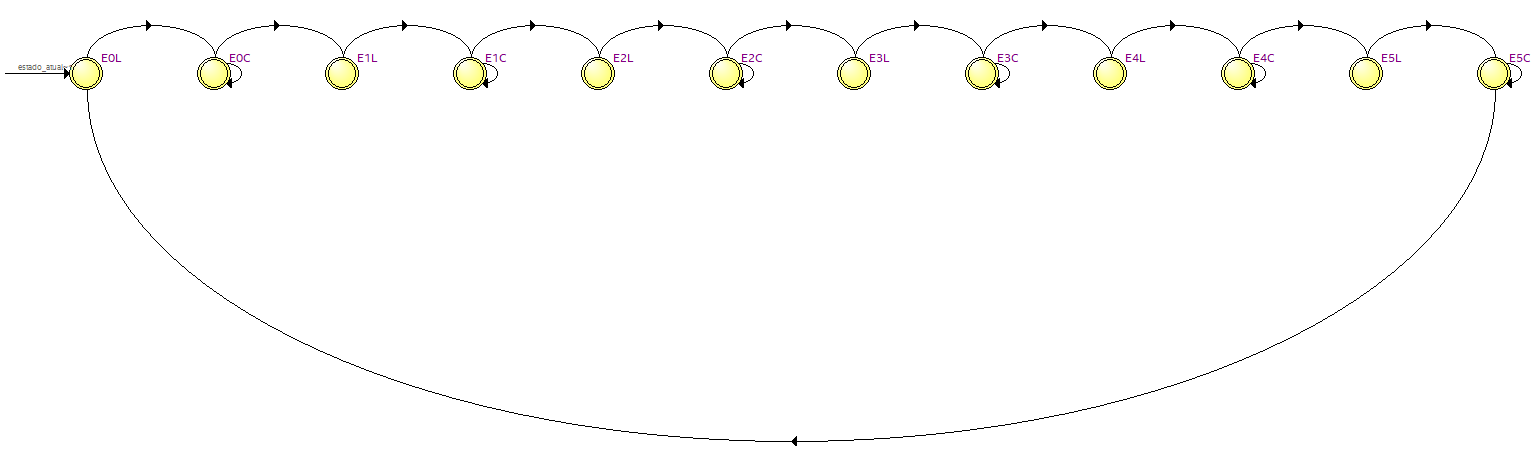
\includegraphics[width=\textwidth]{estados.png}
    \caption{Diagrama de estados da unidade de controle}
    \label{fig:estados}
\end{figure}




\subsection{Simulação}

As Figs. \ref{fig:ct_fd}, \ref{fig:ct_uc} e \ref{fig:ct_completo} mostram as cartas de tempos do Fluxo de Dados, da Unidade de Controle e do Circuito Completo, respectivamente, obtidas pela simulação do circuito.

\begin{figure}[!ht]
    \centering
    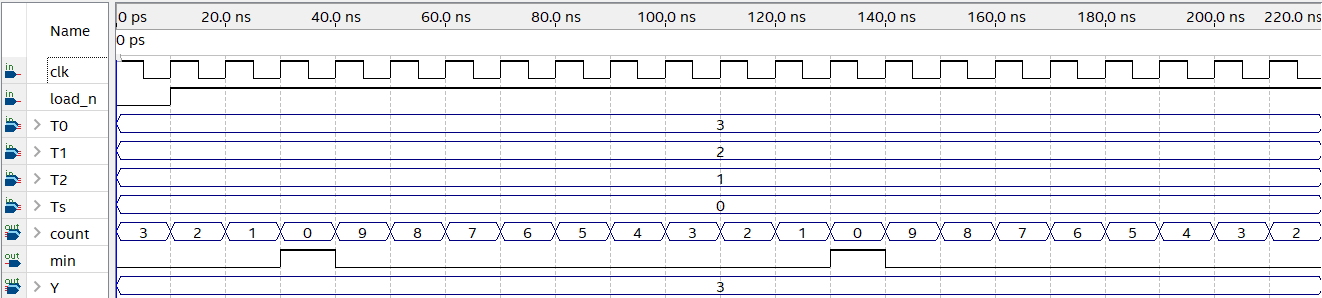
\includegraphics[width=\textwidth]{sem_fd.png}
    \caption{Carta de tempos do Fluxo de Dados}
    \label{fig:ct_fd}
\end{figure}

\begin{figure}[!ht]
    \centering
    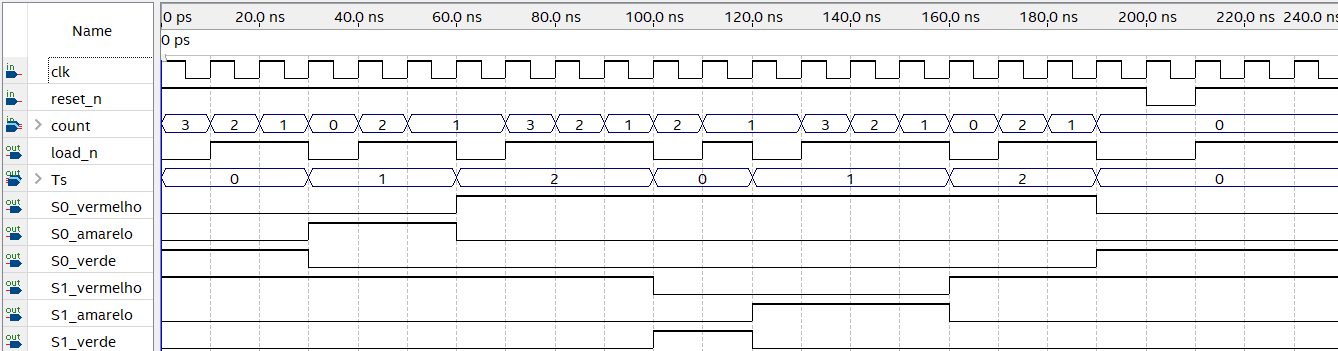
\includegraphics[width=\textwidth]{sem_uc.png}
    \caption{Carta de tempos da Unidade de Controle}
    \label{fig:ct_uc}
\end{figure}

\begin{figure}[!ht]
    \centering
    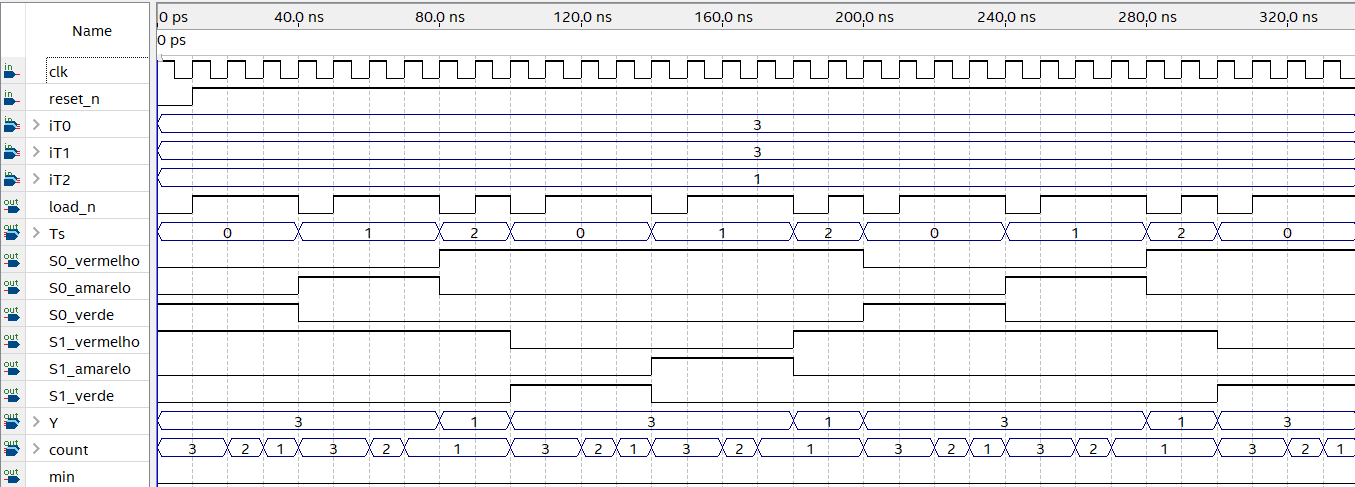
\includegraphics[width=\textwidth]{sem_completo.png}
    \caption{Carta de tempos do Circuito Completo, incluindo Fluxo de Dados e Unidade de Controle}
    \label{fig:ct_completo}
\end{figure}



\subsection{Testes}
\label{sec:teste}

As tabelas de teste foram criadas a partir da simulação e possui os valores esperados para os sinais de saída e depuração. As Tabelas \ref{tab:fd}, \ref{tab:uc} e \ref{tab:completo} mostram as tabelas de testes para o Fluxo de Dados, a Unidade de Controle e o Circuito Completo, respectivamente.


\begin{table}[!ht]
    \centering
    \caption{Tabela de testes do Fluxo de Dados}
    \label{tab:fd}
    \doubleRuleSep
    \begin{tabular}{*{9}{c}}
        \doubleTopRule
        \multicolumn{6}{c}{Entradas} & \multicolumn{2}{c}{Saídas} & Dep.\\
        \cmidrule(lr){1-6}\cmidrule(lr){7-8}\cmidrule(lr){9-9}
        clk & $\n{\textrm{load}}$ & $T_0$ & $T_1$ & $T_2$ & $T_s$ & min &  count & Y \\
        \midrule
        \csvreader[late after line=\\]{fd.csv}{}%
        {\csvcoli & \csvcolii & \csvcoliii & \csvcoliv & \csvcolv & \csvcolvi & \csvcolvii & \csvcolviii &\csvcolix}%
        \doubleBottomRule
    \end{tabular}
\end{table}

\begin{table}[!ht]
    \centering
    \caption{Tabela de testes no Circuito Completo}
    \label{tab:uc}
    \doubleRuleSep
    \begin{tabular}{*{11}{c}}
        \doubleTopRule
        \multicolumn{3}{c}{Entradas} & \multicolumn{8}{c}{Saídas}\\
        \cmidrule(lr){1-3}\cmidrule(lr){4-11}
        clk & $\n{\textrm{rst}}$ & count & $\n{\textrm{load}}$ & $T_s$ & {\color{red}$S_0$} & {\color{orange}$S_0$} & {\color{green}$S_0$} & {\color{red}$S_1$} & {\color{orange}$S_1$} & {\color{green}$S_1$} \\
        \midrule
        \csvreader[late after line=\\]{resultados2.csv}{}%
        {\csvcoli & \csvcolii & \csvcolviii & \csvcolvi & \csvcolvii & \csvcolx & \csvcolxi & \csvcolxii & \csvcolxiii & \csvcolxiv & \csvcolxv}%
        \doubleBottomRule
    \end{tabular}
\end{table}


\begin{table}[!ht]
    \centering
    \caption{Tabela de testes no Circuito Completo}
    \label{tab:completo}
    \doubleRuleSep
    \begin{tabular}{*{15}{c}}
        \doubleTopRule
        \multicolumn{5}{c}{Entradas} &  \multicolumn{4}{c}{Depuração} & \multicolumn{6}{c}{Saídas}\\
        \cmidrule(lr){1-5}\cmidrule(lr){6-9}\cmidrule(lr){10-15}
        clk & $\n{\textrm{rst}}$ & $T_0$ & $T_1$ & $T_2$ & $\n{\textrm{load}}$ & $T_s$ & count & Y & {\color{red}$S_0$} & {\color{orange}$S_0$} & {\color{green}$S_0$} & {\color{red}$S_1$} & {\color{orange}$S_1$} & {\color{green}$S_1$} \\
        \midrule
        \csvreader[late after line=\\]{resultados2.csv}{}%
        {\csvcoli & \csvcolii & \csvcoliii & \csvcoliv & \csvcolv & \csvcolvi & \csvcolvii & \csvcolviii  & \csvcolix & \csvcolx & \csvcolxi & \csvcolxii & \csvcolxiii & \csvcolxiv & \csvcolxv}%
        \doubleBottomRule
    \end{tabular}
\end{table}




\clearpage
% \afterpage{\clearpage}
\subsection{Levantamento dos materiais necessários}
\label{sec:plan_materiais}

\begin{table}[!ht]
    \centering
    \caption{Unidades requeridas para cada CI}
    \label{tab:materiais}
    \doubleRuleSep
    \begin{tabular}{lllrr}
        \doubleTopRule
        Slot & Operação & CI & Un. Requeridas & Un. Disponíveis \\
        \midrule
        1 & Contador & 74190 & 1 & 1\\
        2 & Multiplexador & 74153 & 2 & 2\\
        \doubleBottomRule
    \end{tabular}
\end{table}

Para garantir que o circuito projetado respeite as restrições de montagem, fizemos um levantamento dos recursos necessários para este circuito mostrado na Tabela \ref{tab:materiais}. Ela mostra a quantidade de unidades lógicas requeridas para cada CI utilizado. As especificações de cada CI foi obtido pelos respectivos \emph{datasheets}.




% \newpage
\subsection{Montagem e Depuração}
\label{sec:montagem}

O circuito será montado e depurado por partes. A Tabela \ref{tab:sinais_fd} mostra a correlação dos sinais de depuração e dos LEDS da placa de montagem do fluxo de dados e a Tabela \ref{tab:sinais_uc} mostra a designação dos pinos da unidade de controle. Os sinais de saída (luzes do semáforo) serão mostrados nos LEDS da FPGA. 

\begin{table}[!ht]
    \centering
    \caption{Tabela de correlação dos sinais de depuração com os LEDS da placa de montagem do Fluxo de Dados}
    \label{tab:sinais_fd}
    \doubleRuleSep
    \begin{tabular}{cccc}
        \doubleTopRule
        Sinal & Endereço da Porta & Número do LED & Tipo E/S \\
        \midrule
        $Q_A$ & 74163:14 & LED0 & Saída\\
        $Q_B$ & 74163:13 & LED1 & Saída\\
        $Q_C$ & 74163:12 & LED2 & Saída\\
        $Q_D$ & 74163:11 & LED3 & Saída\\
        $O_A$ & 74163:3 & LED4 & Entrada\\
        $O_B$ & 74163:4 & LED5 & Entrada\\
        $O_C$ & 74163:5 & LED6 & Entrada\\
        $O_D$ & 74163:6 & LED7 & Entrada\\
        \doubleBottomRule
    \end{tabular}
\end{table}


\begin{table}[!ht]
    \centering
    \caption{Tabela de designação de pinos da Unidade de Controle para a placa FPGA DE0-CV com Cyclone
V 5CEBA4F23C7}
    \label{tab:sinais_uc}
    \doubleRuleSep
    \begin{tabular}{rccc}
        \doubleTopRule
        % {} & \multicolumn{2}{c}{GPIO} & FPGA\\
        % \cmidrule(lr){2-3}\cmidrule(lr){4-4}
        Sinal & Código Interface & Código FPGA & Tipo E/S \\
        \midrule
        clk & GPIO\_0\_D0 & N16 & Entrada\\
        $\n{\textrm{reset}}$ & GPIO\_0\_D1 & B16 & Entrada\\
        $\n{\textrm{end}}$ & GPIO\_0\_D3 & C16 & Entrada\\
        $T_0[0]$ & GPIO\_0\_D4 & D17 & Entrada\\
        $T_0[1]$ & GPIO\_0\_D5 & K20 & Entrada\\
        $T_0[2]$ & GPIO\_0\_D6 & K21 & Entrada\\
        $T_0[3]$ & GPIO\_0\_D7 & K22 & Entrada\\
        $T_1[0]$ & GPIO\_0\_D8 & M20 & Entrada\\
        $T_1[1]$ & GPIO\_0\_D9 & M21 & Entrada\\
        $T_1[2]$ & GPIO\_0\_D10 & N21 & Entrada\\
        $T_1[3]$ & GPIO\_0\_D11 & R22 & Entrada\\
        $T_2[0]$ & GPIO\_0\_D12 & R21 & Entrada\\
        $T_2[1]$ & GPIO\_0\_D13 & T22 & Entrada\\
        $T_2[2]$ & GPIO\_0\_D14 & N20 & Entrada\\
        $T_2[3]$ & GPIO\_0\_D15 & N19 & Entrada\\
        $\n{\textrm{load}}$ & GPIO\_1\_D1 & A12 & Saída\\
        offset[0] & GPIO\_1\_D4 & A13 & Saída\\
        offset[1] & GPIO\_1\_D5 & B13 & Saída\\
        offset[2] & GPIO\_1\_D6 & C13 & Saída\\
        offset[3] & GPIO\_1\_D7 & D13 & Saída\\
        $S_0$ vermelho & LEDR2 & W2 & Saída\\
        $S_0$ amarelo & LEDR1 & AA1 & Saída\\
        $S_0$ verde & LEDR0 & AA2 & Saída\\
        $S_1$ vermelho & LEDR5 & Y3 & Saída\\
        $S_1$ amarelo & LEDR4 & N2 & Saída\\
        $S_1$ verde & LEDR3 & N1 & Saída\\
        \doubleBottomRule
    \end{tabular}
\end{table}




\newpage
\section{Resultados}
A implementação do Fluxo de Dados e da Unidade de Controle foram realizadas com sucesso na placa de montagem e na FPGA, respectivamente. Cada um desses componentes foram montados e testados separadamente e os resultados foram comparados com as Tabelas \ref{tab:fd} e \ref{tab:uc}. Após concluídos os testes unitários, o Fluxo de Dados e a Unidade de Controle foram devidamente conectadas e testadas de acordo com a Tabela \ref{tab:completo}. Todas as saídas do circuito estão de acordo com o esperado e nenhuma alteração do planejamento foi realizada durante a montagem. Os resultados dos testes no Circuito Completo estão anotados na coluna ``Check'' da Tabela \ref{tab:resultados}. 


\begin{table}[!ht]
    \centering
    \caption{Resultado dos testes no Circuito Completo}
    \label{tab:resultados}
    \doubleRuleSep
    \begin{tabular}{*{16}{c}}
        \doubleTopRule
        \multicolumn{5}{c}{Entradas} &  \multicolumn{4}{c}{Depuração} & \multicolumn{6}{c}{Saídas}\\
        \cmidrule(lr){1-5}\cmidrule(lr){6-9}\cmidrule(lr){10-15}
        clk & $\n{\textrm{rst}}$ & $T_0$ & $T_1$ & $T_2$ & $\n{\textrm{load}}$ & $T_s$ & count & Y & {\color{red}$S_0$} & {\color{orange}$S_0$} & {\color{green}$S_0$} & {\color{red}$S_1$} & {\color{orange}$S_1$} & {\color{green}$S_1$} & Check \\
        \midrule
        \csvreader[late after line=\\]{resultados2.csv}{}%
        {\csvcoli & \csvcolii & \csvcoliii & \csvcoliv & \csvcolv & \csvcolvi & \csvcolvii & \csvcolviii  & \csvcolix & \csvcolx & \csvcolxi & \csvcolxii & \csvcolxiii & \csvcolxiv & \csvcolxv & \csvcolxvi}%
        \doubleBottomRule
    \end{tabular}
\end{table}



\section{Conclusão}
Neste experimento, usamos a separação Fluxo de Dados e Unidade de Controle em um projeto de semáforos. O Fluxo de Dados foi montado em uma placa de montagem usando CIs TTL e a Unidade de Controle foi implantado em uma FPGA com descrição em VHDL. A conexão entre placa de montagem e FPGA foi feita usando conversores de tensão. Os sinais obtidos pelos testes no circuto estão de acordo com as tabelas de testes previamente elaboradas.


\newpage
\appendix
\section*{Apêndice}
\renewcommand{\thesubsection}{\Alph{subsection}}

\subsection{Descrições VHDL}
\label{ap:vhdl}

% Descrições comentadas dos circuitos comparador e contador em VHDL

\begin{code}
\captionof{listing}{Descrição da Unidade de Controle}
\label{lst:uc}
\vspace{-12pt}
\inputminted[frame=lines, framesep=6pt, framerule=0.5pt, linenos, rulecolor=secondaryColor, breaklines]{VHDL}{unidade_controle.vhd}
\end{code}


% \bibliographystyle{plainnat}
% \bibliography{refs}

\horizonBackCover
\end{document}